\documentclass[11pt]{article}
\usepackage{tikz}
\usetikzlibrary{automata,positioning}
\begin{document}
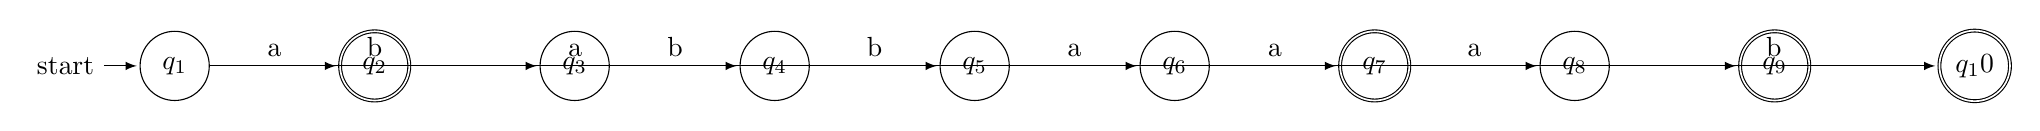
\begin{tikzpicture}[>=latex, shorten >=1pt, node distance=1in, on grid, auto]
% Vertices of automaton
\node [state,initial] (q1) {$q_1$};
\node [state, accepting] (q2) [right=of q1] {$q_2$};
\node [state] (q3) [right=of q2] {$q_3$};
\node [state] (q4) [right=of q3] {$q_4$};
\node [state] (q5) [right=of q4] {$q_5$};
\node [state] (q6) [right=of q5] {$q_6$};
\node [state, accepting] (q7) [right=of q6] {$q_7$};
\node [state] (q8) [right=of q7] {$q_8$};
\node [state, accepting] (q9) [right=of q8] {$q_9$};
\node [state, accepting] (q10) [right=of q9] {$q_10$};
% edges of automaton
\path[->]
(q1) edge node {a} (q2)
(q1) edge node {b} (q3)
(q2) edge node {a} (q4)
(q2) edge node {b} (q5)
(q3) edge node {b} (q6)
(q4) edge node {a} (q7)
(q5) edge node {a} (q8)
(q6) edge node {a} (q9)
(q8) edge node {b} (q10)
;
\end{tikzpicture}
\end{document}
